\documentclass[parskip=full]{scrartcl}

\pdfoutput=1

\title{Increasing the Effectiveness of Active Learning:\\ 
	\LARGE{Introducing Artificial Data Generation in Active Learning for Land Use/Land Cover Classification}}
\author{
	Joao Fonseca\(^{1}\), Georgios Douzas\(^{1}\), Fernando Bacao\(^{1*}\) 
	\\
	\small{\(^{1}\)NOVA Information Management School, Universidade Nova de Lisboa}
	\\
	\small{*Corresponding Author}
	\\
	\\
	\small{Postal Address: NOVA Information Management School, Campus de Campolide, 1070-312 Lisboa, Portugal}
	\\
	\small{Telephone: +351 21 382 8610}
}

\usepackage{breakcites}
\usepackage{float}
\usepackage{graphicx}
\usepackage{subcaption}
\usepackage{geometry}
\geometry{
	a4paper,
	left=18mm,
	right=18mm,
	top=8mm,
}
\usepackage{amsmath}
\newcommand{\inlineeqnum}{\refstepcounter{equation}~\mbox{(\theequation)}}
\usepackage{enumitem}
\usepackage[ruled,vlined]{algorithm2e}
\usepackage{booktabs}
\usepackage{pgfplotstable}
\pgfplotsset{compat=1.14}
\usepackage{longtable}
\usepackage{tabu}
\usepackage{hyperref}
\date{}

\begin{document}

\maketitle

\begin{abstract}
    In remote sensing, Active Learning (AL) has become an important technique
    to collect informative ground truth data ``on-demand'' for supervised
    classification tasks.  In spite of its effectiveness, it is still
    significantly reliant on user interaction, which makes it both expensive
    and time consuming to implement.  Most of the current literature focuses on
    the optimization of AL by modifying the selection criteria, the chooser
    and/or predictors used.  Although improvements in these areas will result
    in more effective data collection, the use of artificial data sources to
    reduce human-computer interaction remains unexplored. In this paper, we
    introduce a new component to the typical AL framework, the data generator,
    a source of artificial data to reduce the amount of user-labeled data
    required in AL\@.  The implementation of the proposed AL framework is done
    using SMOTE and Geometric SMOTE as data generators.  We compare the new AL
    framework to the original one using similar acquisition functions and
    predictors over three AL-specific performance metrics in seven benchmark
    datasets. We show that this modification to the AL framework significantly
    reduces cost and time requirements for a successful AL implementation in
    the context of remote sensing. 
\end{abstract}

\section{Introduction}~\label{sec:introduction}

The technological development of air and space borne sensors, as well as the
increasing number of remote sensing missions have allowed the continuous
collection of large amounts of high quality remotely sensed data. This data is
often composed of multi and hyper spectral satellite imagery, essential for
numerous applications, such as Land Use/Land Cover (LULC) change detection,
ecosystem management~\cite{Nagai2020}, agricultural
management~\cite{Huang2018}, water resource management~\cite{Wang2018}, forest
management, and urban monitoring~\cite{Khatami2016}. Despite LULC maps being
essential for most of these applications, their production still a challenging
task~\cite{Gavade2019, Wulder2018}. They can be updated using either one of the
following strategies:

\begin{enumerate}
    \item Photo-interpreted. Consists of evaluating a patch's LULC class based
        on orthophoto and satellite image
        interpretation~\cite{costa2020introducing}. This method guarantees a
        decent level of accuracy, as it is dependent on the interpreter's
        expertise and human error. Typically, it is an expensive,
        time-consuming task that requires the expertise of a photo-interpreter.
        This task is also frequently applied to obtain ground-truth labels for
        training and/or validating Machine Learning (ML) algorithms for related
        tasks~\cite{vermote2020remote, COSTANTINO2020}. 
    \item Automated mapping. It is based on the usage of a ML method or a
        combination of methods in order to obtain an updated LULC map. The
        development of a reliable automated method is still a challenge among
        the ML and remote sensing community, since the efficacy of existing
        methods vary across applications and geographical
        areas~\cite{Gavade2019}. Typically, this method requires the existence
        of ground-truth data, which is frequently outdated or nonexistent for
        the required time frame~\cite{Nagai2020}. On the other hand, employing
        a ML method provides readily available and relatively inexpensive LULC
        maps. The increasing quality of state-of-the-art classification methods
        have motivated the application and adaptation of these methods in this
        domain~\cite{Maxwell2018}.
    \item Hybrid approaches. They employ photo-interpreted data to augment the
        training dataset and improve the quality of automated
        mapping~\cite{Ruzicka2020}. It attempts to accelerate the
        photo-interpretation process by selecting a smaller sample of the study
        area to be interpreted. The goal is to minimize the inaccuracies found
        in the LULC map by supplying high-quality ground-truth data to the
        automated method. The final (photo-interpreted) dataset consists of
        only the most informative samples, i.e., patches that are typically
        difficult to classify for a traditional automated mapping
        method~\cite{Liu2020}. 
\end{enumerate}

The latter method is best know as AL\@. It is especially useful whenever there
is an absence of ground-truth data and/or the mapping region does not contain
updated LULC maps~\cite{Su2020}. In a context of limited sample-collection
budget, the collection of the most informative samples capable of optimally
increasing the classification accuracy of a LULC map is of particular
interest~\cite{Su2020}. AL attempts to minimize the human-computer interaction
involved in photo-interpretation by selecting the data points to include into
the annotation process. These data points are selected based on an uncertainty
measure and represent the points close to the decision borders. Afterwards,
they are passed on for photo-interpretation and added to the training dataset,
while the points with the lowest uncertainty values are ignored for
photo-interpretation and classification. This process is iterated until a
convergence criterion is reached~\cite{Pasolli2016}. 

The relevant work developed within AL is described in detail in
Section~\ref{sec:al-sota}. The research attempts to address some of the
challenges found in AL, mainly inherited from automated and photo-interpreted
mapping: mapping inaccuracies and time consuming human-computer interactions.
These challenges have different sources:

\begin{enumerate}
    \item Human error. The involvement of photo-interpreters in the data
        labeling step carries an additional risk to the creation of LULC
        patches. The minimum mapping unit being considered, as well as the
        quality of the orthophotos and satellite images being used, are some of
        the factors that may lead to the overlooking of small-area LULC patches
        and label-noisy training data~\cite{Pelletier2017}.
    \item High-dimensional datasets. The amount of bands (i.e., features)
        present in multi and hyper spectral images introduce an increased level
        of complexity in the classification step~\cite{Stromann2020}. These
        datasets are often prone to the Hughes phenomenon, also known as the
        curse of dimensionality. 
    \item Class separability. Producing an LULC map considering classes with
        similar spectral signatures makes them difficult to
        separate~\cite{Alonso-Sarria2019}. A lower pixel resolution of the
        satellite images may also imply mixed-class pixels, which may lead to
        both lower class separability as well as higher risk of human error.
    \item Existence of rare land cover classes. The varying morphologies of
        different geographical regions naturally implies an uneven distribution
        of land cover classes~\cite{Feng2018}. This is particularly relevant in
        the context of AL:\@ the data selection method is based on a given
        uncertainty measure over data points whose class label is unknown.
        Consequently, AL's iterative process of data selection may disregard
        wrongly classified land cover areas belonging to a minority class.
\end{enumerate}

Research developed in the field of Active Learning typically focus on the
reduction of human error by minimizing the human interaction with the process
through the development of more efficient choosers and selection criteria
within the generally accepted AL framework.  Concurrently, the problem of rare
land cover classes is rarely addressed. This is a frequent problem in the ML
community, known as the Imbalanced Learning problem. This problem exists
whenever there is an uneven between-class distribution in the
dataset~\cite{Chawla2004}. Specifically, most classifiers attempt to optimize
metrics such as overall accuracy, which are designed to work primarily with
balanced datasets. Consequently, these metrics tend to introduce a bias towards
the majority class by attributing an importance to each class proportional to
its relative frequency~\cite{Maxwell2018}. As an example, such a classifier
could achieve an overall accuracy of 99\% on a binary dataset where the
minority class represents 1\% of the overall dataset and still be deemed
useless. A number of methods have been developed to deal with this problem.
They can be categorized into three different types of
approaches~\cite{Fernandez2013,Kaur2019}. Cost-sensitive solutions perform
changes to the cost matrix in the learning phase. Algorithmic level solutions
modify specific classifiers to reinforce learning on minority classes.
Resampling solutions modify the dataset by removing majority samples and/or
generating artificial minority samples. The latter is independent from the
context and can be used alongside any classifier. We will focus on artificial
data generation techniques, presented in Section~\ref{sec:ovs-sota}.

In this paper, we propose a novel AL framework to address two limitations
commonly found in the literature: minimize human-computer interaction and
reduce the class imbalance bias. This is done with the introduction of an
additional component in the iterative AL procedure (the generator), used to
generate artificial data to both balance and augment the training dataset. The
introduction of this component is expected to reduce the number of iterations
required until convergence of the predictor's quality.

This paper is organized as follows: Section~\ref{sec:introduction} exposes the
problem and its context, Sections~\ref{sec:al-sota} and~\ref{sec:ovs-sota}
describe the state of the art in AL and Oversampling techniques,
Section~\ref{sec:proposed-method} exposes the proposed method,
Section~\ref{sec:methodology} covers the datasets, evaluation metrics, ML
classifiers and experimental procedure, Section~\ref{sec:results} presents the
experiment's results and Section~\ref{sec:conclusion} reports the
conclusions drawn from our findings.

\section{Active Learning Approaches}~\label{sec:al-sota}

As the amount of unlabeled data increases, the interest and practical
usefulness of AL follows that trend~\cite{Kottke2017}. AL is used as the
general definition of frameworks aiming to train a learning system in multiple
steps, where a set of new data points are chosen and added to the training
dataset each time~\cite{Ruzicka2020}. Typically, an AL framework is composed of
10 elements~\cite{Sverchkov2017,Su2020,Ruzicka2020}:

\begin{enumerate}
    \item Data source. In the context of LULC classification, the data source
        is usually a hyper/multi-spectral image, a Synthetic-aperture radar
        (SAR) image, or a composite image.
    \item Unlabeled dataset. Consists of a sample of the original data source.
        It is used in combination with the chooser and the selection criterion
        to retrieve uncertainty estimates on each iteration.
    \item Initial training sample. It is a small sample of the unlabeled
        dataset, used to initiate the first AL iteration. The size of the
        initial training sample normally varies between no observations at all
        and 10\%~\cite{Li2013}.
    \item Augmented training dataset. This dataset is the concatenation of the
        labeled initial training sample along with the datasets labeled by the
        oracle in past iterations.
    \item Uncertainty map. The dataset containing the highest uncertainty
        points/patches to be labeled by the oracle.
    \item Oracle. An external entity to which the uncertainty map is presented
        to. The oracle is responsible for annotating unlabeled samples to be
        added to the augmented dataset. In remote sensing, the oracle is
        typically a photo-interpreter, as is the case in~\cite{li2020}. Some of
        the research also refers to the oracle as the
        \textit{supervisor}~\cite{Su2020, Shrivastava2021}.
    \item Chooser. Produces the class probabilities for each unlabeled sample.
        This is a classifier trained using the augmented dataset. It is used to
        estimate the class probabilities for each sample over the unlabeled
        dataset.
    \item Selection criterion. It quantifies the chooser's uncertainty level
        for each sample belonging to the unlabeled dataset. It is typically
        based on the class probabilities assigned by the chooser. In some
        situations, the chooser and the selection criterion are grouped
        together under the concept \textit{acquisition
        function}~\cite{Ruzicka2020} or \textit{query function}~\cite{Su2020}.
        Some of the literature refers to the selection criterion by using the
        concept \textit{sampling scheme}~\cite{Liu2020}.
    \item Predictor. The classifier used to infer the land cover classes for
        the final output map. Once a stopping criterion is met, the classifier
        is trained using the augmented dataset and the LULC classes are
        inferred from the data source.
    \item Prediction output. In the context of LULC classification, the
        prediction output is the estimated LULC map raster.
\end{enumerate}

Figure~\ref{fig:al_typical} schematizes the steps involved in a complete AL
iteration. For a better context within the remote sensing domain, the
prediction output is identified as the LULC map. This framework starts by
collecting unlabeled data from the original data source. It is used to generate
a random initial training sample and is labeled by the oracle. In practical
applications, the oracle is frequently a group of
photo-interpreters~\cite{Kottke2017}. The chooser is trained on the resulting
dataset and is used to predict the class probabilities on the unlabeled
dataset. The class probabilities are fed into a selection criterion to estimate
the prediction's uncertainty, out of which the samples with the highest
uncertainty will be selected. This calculation is motivated by the absence of
labels in the uncertainty dataset. Therefore, it is impossible to estimate the
prediction's accuracy in a real case scenario. The iteration is completed when
the selected points are tagged by the oracle and added to the training dataset
(i.e., the augmented dataset). 

\begin{figure}[htb]
	\centering
	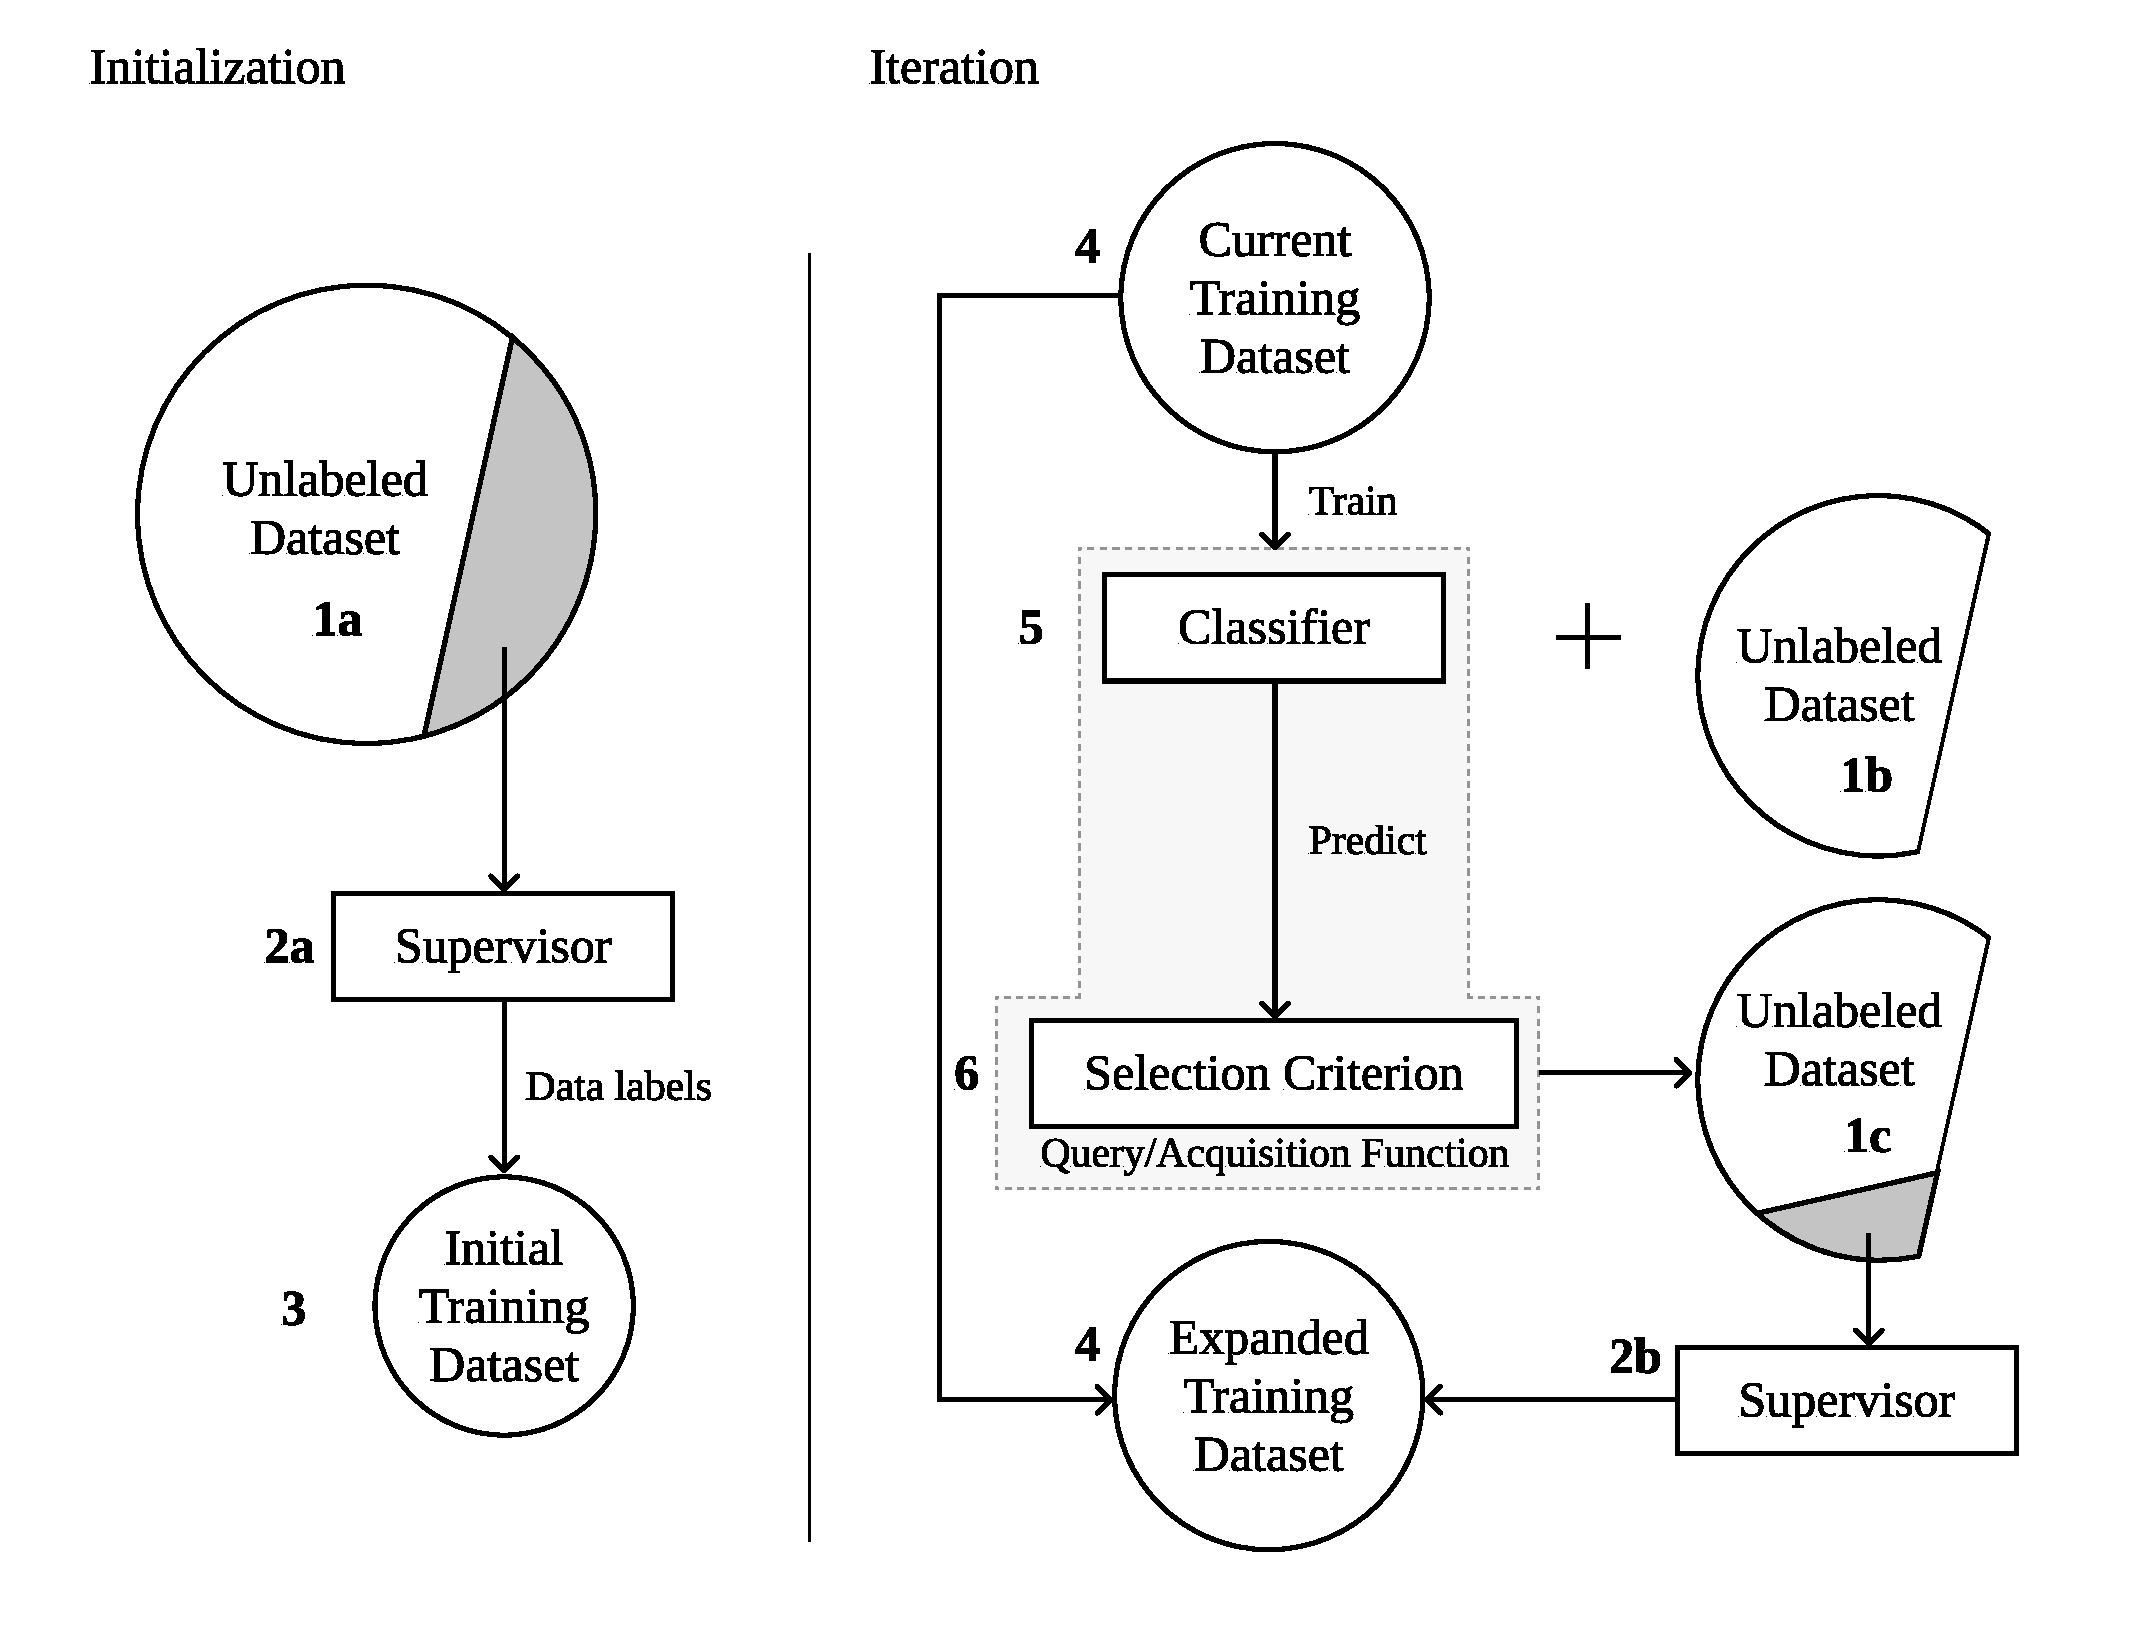
\includegraphics[width=.85\linewidth]{../analysis/al_typical}
	\caption{Diagram depicting the typical AL framework. Although the chooser
        and predictor are presented as separate entities, they are frequently
        the same classifier.
    }~\label{fig:al_typical}
\end{figure}

A common challenge found in AL tasks is ensuring the consistency of AL over
different initializations~\cite{Kottke2017}. There are two factors involved in
this phenomenon. On the one hand, the implementation of the same method over
different initializations may result in significantly different initial
training samples, amounts to varying accuracy curves. On the other hand, the
lack of a robust selection criterion and/or chooser may also result in
inconsistencies across AL experiments with different initializations. This
phenomenon was observed and documented in a LULC classification context
in~\cite{tuia2011using}.

Selecting an efficient selection criterion is particularly important to find
the samples closest to the decision border (i.e., samples difficult to
classify)~\cite{Shrivastava2021}. Therefore, most of AL related studies focus
on the design of the query/acquisition function~\cite{Su2020}.

\subsection{Non-informed selection criteria}

Only one non-informed selection criterion was found. Random sampling selects
unlabeled samples without considering any external information produced by the
chooser. Since the method for selecting the unlabeled samples is random, this
method disregards the usage of a chooser and is comparatively worse than any
other selection criterion. Although, random sampling is still a powerful
baseline method~\cite{Cawley2011}. Generally, different AL initializations
return high performance variability~\cite{Kottke2017}. When this happens, the
analysis of the mean performances over multiple repetitions is not of interest
on its own. Instead, it is preferable to do pairwise comparison of different
methods along with their corresponding variances. 

\subsection{Ensemble-based selection criteria}

Ensemble disagreement is based on the class predictions of a set of
classifiers.  The disagreement between all the predictions for a given
observation is a common measure for uncertainty, although computationally
inefficient~\cite{Ruzicka2020,Pasolli2016}. It is calculated using the set of
classifications over a single observation, given by the number of votes
assigned to the most frequent class~\cite{Shrivastava2021}. This method was
implemented successfully for complex applications such as deep active
learning~\cite{Ruzicka2020}.

Multiview~\cite{Muslea2006} consists on the training of multiple independent
classifiers using different views, which correspond to the selection of subsets
of features or observations in the dataset. Therefore, it can be seen as a
bootstrap aggregation (bagging) ensemble disagreement method. It is represented
by the maximum disagreement score out of set of disagreements calculated for
each view~\cite{Shrivastava2021}. A lower value for this metric means a higher
classification uncertainty. Multiview-based maximum disagreement has been
successfully applied to hyper-spectral image classification in~\cite{Di2012}
and~\cite{Zhou2014}.

An adapted disagreement criterion for an ensemble of $k$-nearest neighbors has
been proposed in~\cite{Pasolli2016}. This method employs a $k$-nearest
neighbors classifier and computes an instance's classification uncertainty
based on the neighbors' class frequency using the maximum disagreement metric
over varying values for $k$. As a result, this method is comparable to
computing the dominant class' score over a weighted $k$-nearest neighbors
classifier. This method was also used on a multimetric active learning
framework~\cite{Zhang2016}.

Another relevant ensemble-based selection criterion is the binary random
forest-based query model~\cite{Su2020}. This method employs a one-versus-one
ensemble method to demonstrate an efficient data selection method using the
estimated probability of each binary random forest and determining the
classification uncertainty based on the probabilities closest to 0.5 (i.e., the
least separable pair of classes are used to determine the uncertainty value).
Although, this study fails to compare the proposed method with other benchmark
methods, such as random sampling.

\subsection{Entropy-based criteria}

A number of contributions have focused on entropy-based querying. The
application of entropy is common among active deep learning
applications~\cite{Aghdam2019}, where the training of an ensemble of
classifiers is often too expensive. The measure of entropy is formulated as
follows:

\begin{equation}\label{eq:entropy}
    H(x_i) = \sum_{\omega=1}^{N_i}{p(y_{i}^{*}=\omega|x_i)}\log_2[p(y_{i}^{*}=\omega|x_i)]
\end{equation}

The measurement of entropy $H$ is based on the observed probability
$p(y_{i}^{*}=\omega|x_i)$ of obtaining class $\omega$ as the predicted class
label $y_{i}^{*}$, where $N_i$ is the number classes predicted for observation
$x_i$.

Entropy query-by-bagging (EQB), also defined as maximum entropy~\cite{Liu2020},
is an ensemble approach of the entropy selection criterion, originally proposed
in~\cite{Tuia2009}. This strategy uses the set of predictions produced by the
ensemble classifier to calculate those many entropy measurements. The estimated
uncertainty measure for one sample is given by the maximum entropy within that
set. EQB was observed to be an efficient selection criterion.
Specifically,~\cite{Shrivastava2021} applied EQB on hyper-spectral remote
sensing imagery using Support Vector Machines (SVM) and Extreme Learning
Machines (ELM) as choosers, achieving optimal results when combining EQB with
ELM\@. Another study successfully implemented this method on an active deep
learning application~\cite{Liu2020}. Another study improved over this method
with a normalized EQB selection criterion~\cite{Copa2010}.

\subsection{Other relevant criteria}

Margin Sampling is a SVM-specific criterion, based on the distance of a given
point to the SVM's decision boundary~\cite{Shrivastava2021}. This method is
less popular than the remaining methods because it is limited to one type of
chooser (SVMs). One extension of this method is the multiclass level
uncertainty~\cite{Shrivastava2021}, calculated by subtracting the observation's
distance to the decision boundaries of the two most probable
classes~\cite{Demir2011}.

The Mutual Information-based (MI) criterion selects the new training samples by
maximizing the mutual information between the classifier and class labels in
order to select samples from regions that are difficult to classify. Although
this method is commonly used, it is frequently outperformed by the breaking
ties selection criterion~\cite{Li2011,Liu2018}.

The breaking ties (BT) selection criterion was originally introduced
in~\cite{Luo2003}. It is formulated as follows:

\begin{equation}\label{eq:breaking_ties}
    BT(x_i) = \arg \min_{x_i, i \in S_u}\{ \max_{\omega \in N}{p(y_{i}^{*}=\omega|x_i)} -
    \max_{\omega \in N\setminus\{\omega^{+}\}}{p(y_{i}^{*}=\omega|x_i)}\}
\end{equation}

Which is the subtraction of the probabilities of the two most likely classes.
Another related method is Modified Breaking Ties scheme (MBT), which aims at
finding the samples containing the largest probabilities for the dominant
class~\cite{Liu2018,Li2013a}

Another type of selection criteria identified is the loss prediction
method~\cite{Yoo2019}. This method replaces the selection criterion with a
predictor whose goal is to estimate the chooser's loss for a given
prediction. This allows the new classifier to estimate the prediction loss on
unlabeled observations and select the ones with the highest predicted loss.

Some of the literature fails to specify the strategy employed, although
inferring it is generally intuitive. For example,~\cite{Ertekin2007}
successfully used AL to address the imbalanced learning problem. They employed
an ensemble of SVMs as the chooser and predictor, as well as an ensemble-based
selection criterion. All of the research found related to this topic focused on
the improvement of AL through modifications on the selection criterion, chooser
or predictor. None of these publications proposed significant variations to the
original AL framework.

\section{Artificial Data Generation Approaches}~\label{sec:ovs-sota}

The generation of artificial data is a common approach to address imbalanced
learning tasks~\cite{Kaur2019}, as well as improving the effectiveness of
supervised learning tasks~\cite{DeVries2017}. In recent years some
sophisticated data generation approaches were found. Although, the scope of
this work is to propose the integration of a generator within the AL
framework. To do this, we will focus on heuristic data generation approaches,
specifically, oversamplers.

Heuristic data resampling methods employ local and/or global information to
generate new, relevant, non-duplicated instances. These methods are most
commonly used to populate minority classes and balance the between-class
distribution of a dataset. The Synthetic Minority Oversampling Technique
(SMOTE)~\cite{Chawla2002} was the first heuristic oversampling algorithm to be
proposed. The simplicity and effectiveness of this method contributes to its
prevailing popularity. It generates a new instance $\overrightarrow{z}$ through
a linear interpolation of a randomly selected minority-class observation
$\overrightarrow{x}$ and one of its randomly selected $k$-nearest neighbors
$\overrightarrow{y}$ such that $\overrightarrow{z} = \alpha\overrightarrow{x} +
(1-\alpha)\overrightarrow{y}$ where $\alpha$ is a random float between 0 and 1,
as shown in Figure~\ref{fig:data_generation}. 

\begin{figure}[H]
	\centering
	\includegraphics[width=\linewidth]{../analysis/data_generation}
    \caption{Examples of SMOTE and G-SMOTE generation process. SMOTE randomly
        selects sample $\protect\overrightarrow{x}$ and one of its nearest
        neighbors $\protect\overrightarrow{y}$ to produce sample
        $\protect\overrightarrow{z}$. Noisy sample
        $\protect\overrightarrow{b}$ is generated with SMOTE using points
        $\protect\overrightarrow{a}$ and $\protect\overrightarrow{c}$.  Sample
        $\protect\overrightarrow{p}$ and one of its nearest neighbors
        $\protect\overrightarrow{q}$ are used by G-SMOTE to originate sample
        $\protect\overrightarrow{r}$.
    }~\label{fig:data_generation}
\end{figure}

The implementation of SMOTE for LULC classification tasks has been found to
improve the quality of the predictors used~\cite{Jozdani2019,Bogner2018}.
Despite its popularity, its drawbacks motivated the development of other
oversampling methods~\cite{Douzas2019}:

\begin{enumerate}
    \item Generation of noisy samples due to the selection of $k$-nearest
        neighbors and initial observation. The selection of a sample and/or
        neighboring sample located inside a majority class region may produce
        artificial samples within that region and amplify noisy data.
        Borderline-SMOTE~\cite{Han2005} is a modification of SMOTE in which
        only the minority examples near the borderline are over-sampled. This
        method avoids the generation of noisy samples by disregarding minority
        samples located in a majority class region as well as samples distant
        from the decision borders. The Adaptive Synthetic Sampling approach
        (ADASYN)~\cite{HaiboHe2008} uses a density distribution ratio to
        address this limitation and focus the artificial data generation on
        minority class regions that are more difficult to classify.
    \item Generation of noisy instances due to the use of observations from two
        different minority class clusters. Choosing a minority sample
        $\overrightarrow{a}$ and one of its nearest neighbors
        $\overrightarrow{b}$ belonging to a different minority cluster may lead
        to the generation of a sample $\overrightarrow{c}$ located within the
        two classes, as shown in Figure~\ref{fig:data_generation}. K-means
        SMOTE~\cite{Douzas2018} and Self-Organizing map oversampling
        (SOMO)~\cite{Douzas2017} reduce this effect by oversampling minority
        class samples within the same clusters.
    \item Generation of nearly duplicated instances. The linear interpolation
        of parent samples that are close to each other produces an artificial
        sample with similar properties as its parents. Geometric SMOTE
        (G-SMOTE)~\cite{Douzas2019} introduces a modification of the SMOTE
        algorithm in the data generation mechanism to produce artificial
        samples with higher variability.
\end{enumerate}

The G-SMOTE algorithm is introduced as a generalization of the vanilla SMOTE\@.
Instead of generating artificial data as a linear combination of the parent
samples, it is done within a deformed, truncated hyper-spheroid. G-SMOTE
generates an artificial sample $\overrightarrow{r}$ within a hyper-spheroid
$H$, formed by selecting a minority sample $\overrightarrow{p}$ and one of its
nearest neighbors $\overrightarrow{q}$, as shown in
Figure~\ref{fig:data_generation}. The truncation and deformation parameters
define the shape of the spheroid's geometry. The method also modifies the
selection strategy for the $k$-nearest neighbors, accepting the generation of
artificial samples using observations from different classes. G-SMOTE has shown
superior performance when compared with other oversampling methods for LULC
classification tasks, regardless of the classifier used~\cite{Douzas2019class}.

\section{Proposed method}~\label{sec:proposed-method}

Within the literature identified, most of the work developed in the AL domain
revolved around improving the quality of the chooser, predictor and/or
selection criterion. Although these methods allow earlier convergence of the AL
iterative process, the impact of these methods are only observed between
iterations. Consequently, none of these contributions focused on the
definition of decision borders within iterations. The method proposed in this
paper modifies the AL framework by introducing an artificial data generation
step within AL's iterative process. We define this component as the generator
and is intended to be integrated into the AL framework as shown in
Figure~\ref{fig:al_new}. 

\begin{figure}[htb]
	\centering
	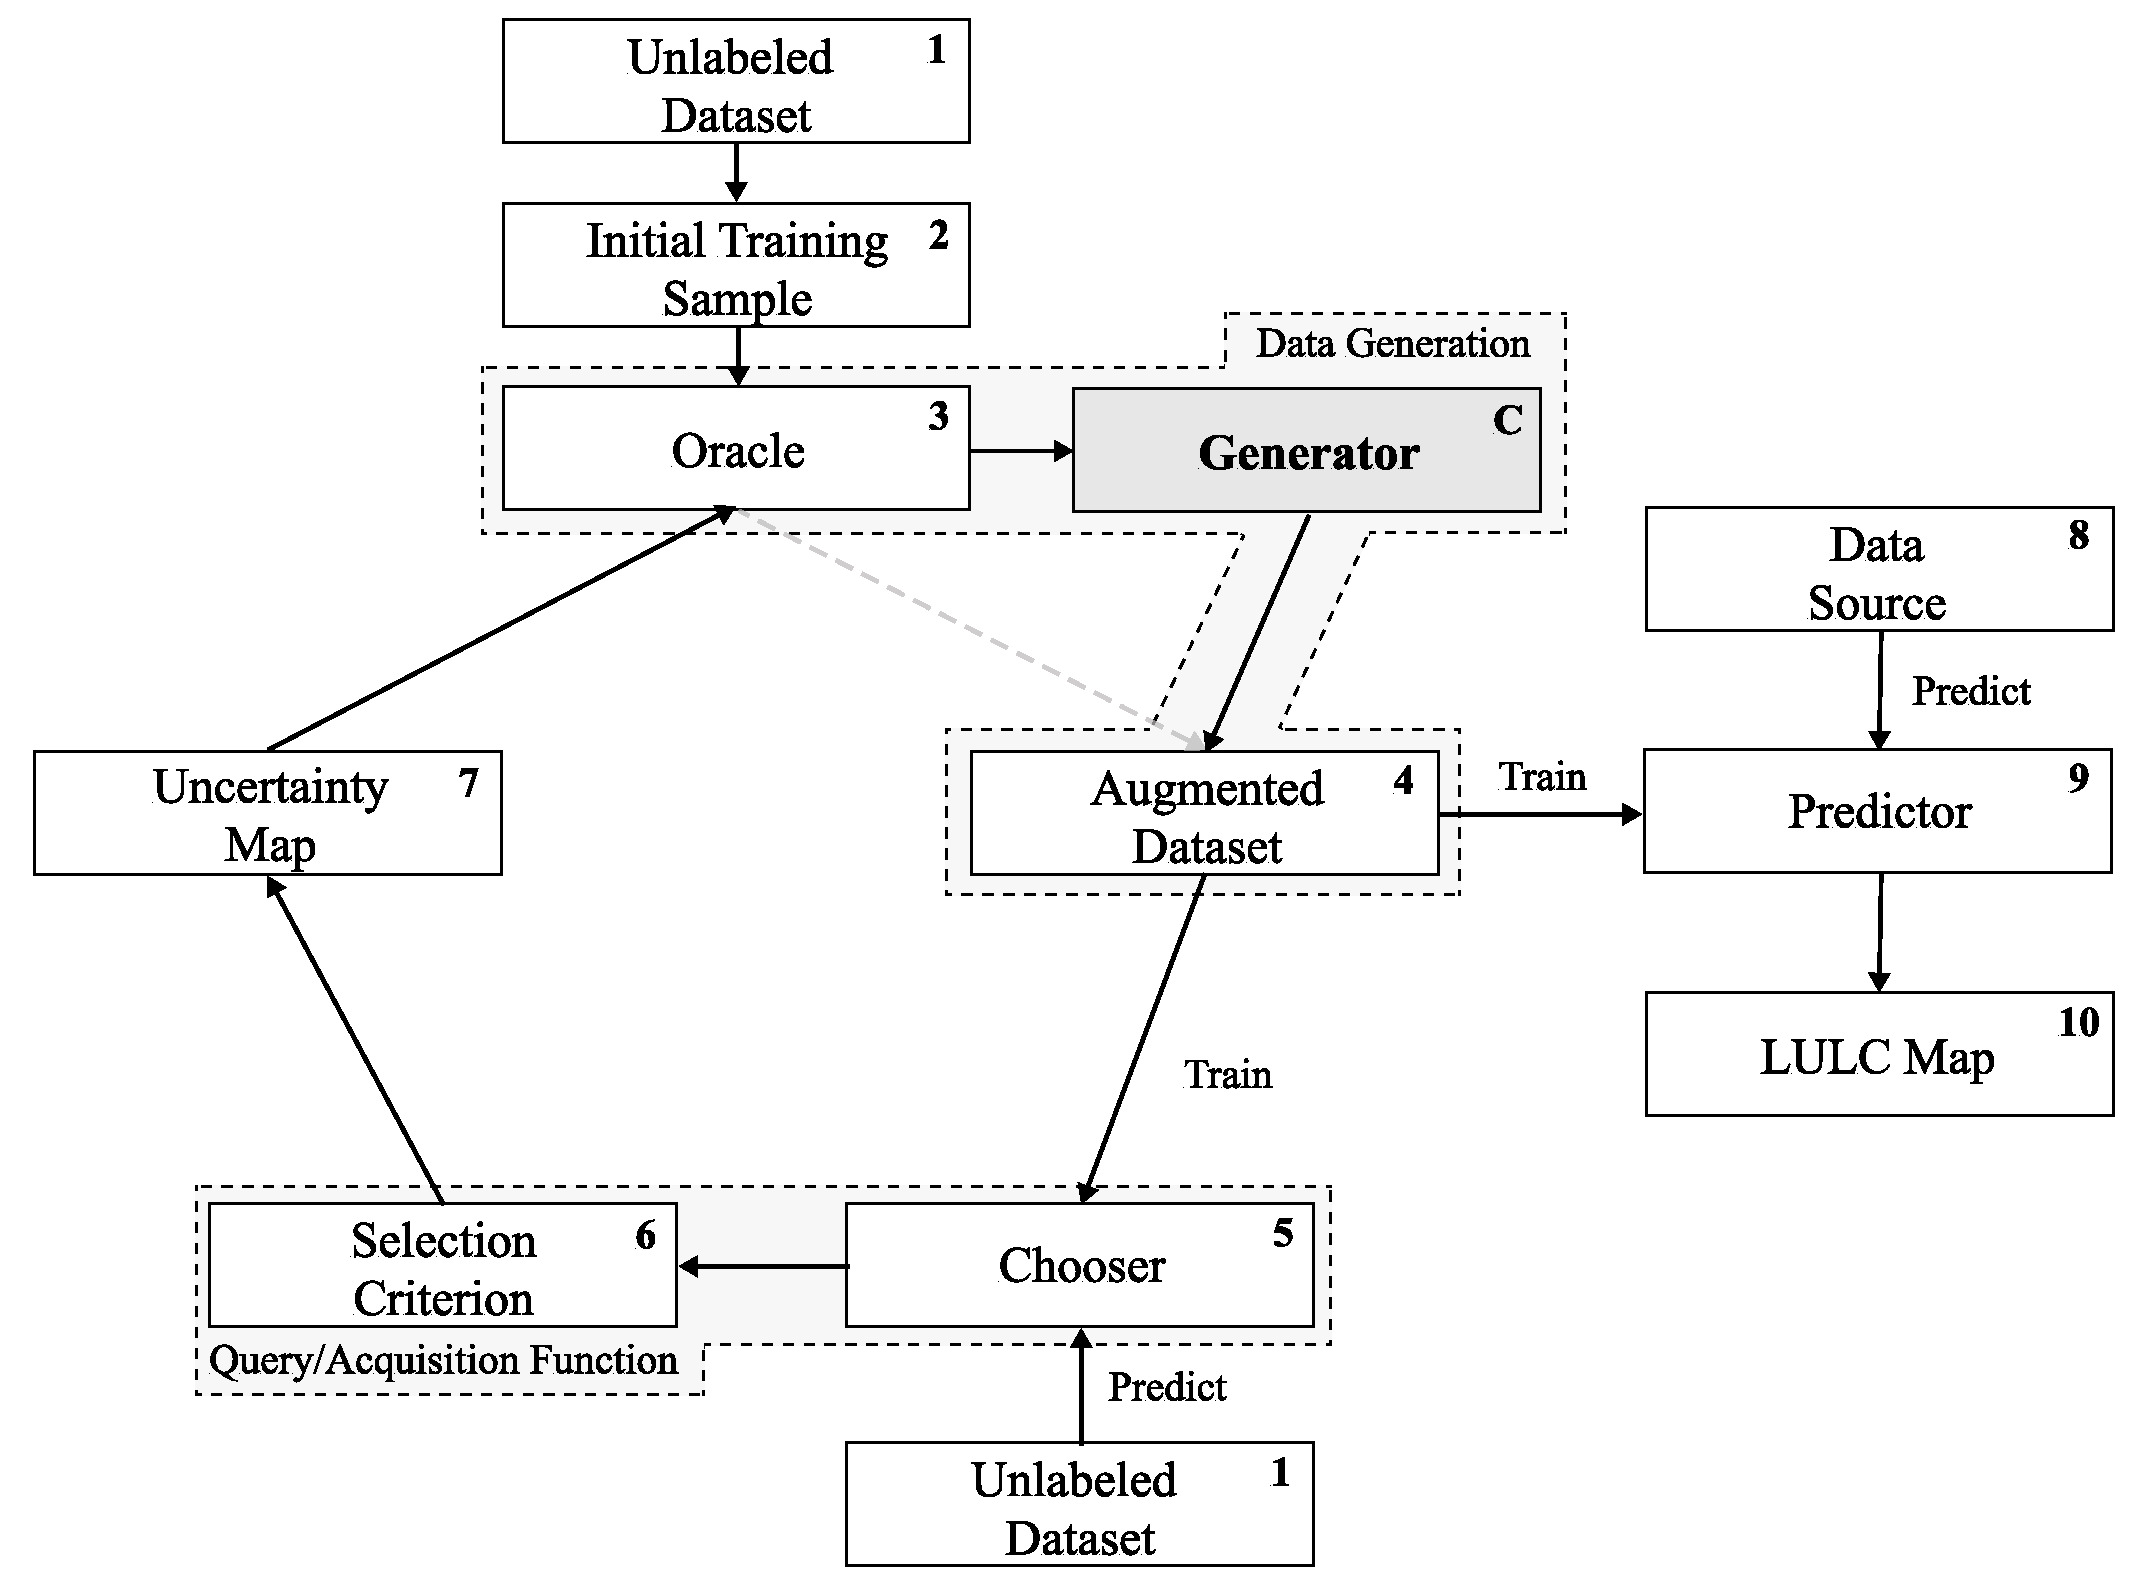
\includegraphics[width=.85\linewidth]{../analysis/al_new}
    \caption{Proposed AL framework. The data generation mechanism is
        represented as the generator, which is used to complete the data
        generation phase. The remaining steps are left unchanged.
    }~\label{fig:al_new}
\end{figure}

This method leverages the capability of artificial data to introduce more data
variability into the augmented dataset and facilitate the chooser's training
phase with a more consistent definition of the decision boundaries at each
iteration. Therefore, any algorithm capable of producing artificial data, be
it agnostic or specific to the domain, can be employed. The artificial data is
only used to train the classifiers involved in the process (chooser and
predictor) and is discarded once the chooser's training phase is completed.
The remaining steps in the AL framework remain unchanged. This method is
addressed towards the limitations found in the previous sections: 

\begin{enumerate}
    \item The convergence of the predictor's performance should be anticipated
        with the clearer definition of the decision boundaries across
        iterations.
    \item Annotation cost is expected to reduce as the need for labeled
        observations reduces along with the early convergence of the
        classification performance.
    \item The class imbalance bias observed in typical classification tasks, as
        well as in AL is mitigated by balancing the class frequencies at each
        iteration.
\end{enumerate}

Although the performance of this method is shown within a LULC classification
context, the proposed framework is independent from the domain. The high
dimensionality of remotely sensed imagery make its classification particularly
challenging when the availability of labeled data is scarce and/or comes at a
high cost, being subjected to the curse of dimensionality. Consequently, it is
a relevant and appropriate domain to test this method.

\section{Methodology}~\label{sec:methodology}

In this section we describe the datasets, evaluation metrics, oversamplers,
classifiers, software used and the procedure developed. We demonstrate the
proposed method's efficiency over 7 datasets, sampled from publicly available,
well-known benchmark remote sensing landscapes frequently found in the
literature. The datasets and sampling strategy are described in
Subsection~\ref{sec:datasets}. On each of these datasets, we implement 3
different classifiers over the entire training set to estimate the optimal
classification performance, the original AL framework as the baseline
reference and the proposed method using two different generators, described in
Subsection~\ref{sec:machine_learning_algorithms}. The metrics used to estimate
the performance of these algorithms are described in
Subsection~\ref{sec:evaluation_metrics}. Finally, the experimental procedure is
described in Subsection~\ref{sec:experimental_procedure}. 

Our methodology focuses on two objectives: (1) Comparison of optimal
classification performance among active learners and traditional supervised
learning and (2) Comparison of classification convergence efficiency across AL
frameworks.

\subsection{Datasets}~\label{sec:datasets}

The datasets used were extracted from publicly available hyperspectral scenes.
Additionally, all datasets were collected using the same sampling procedure.
The description of the hyperspectral scenes used in this study is provided in
Table~\ref{tab:rs_scene_description}. These scenes were chosen because of their
popularity in the research community and their high baseline classification
scores. Consequently, demonstrating an outperforming method in this context is
particularly challenging and valuable.

\pgfplotstabletypeset[
	begin table=\begin{longtable},
		end table=\end{longtable},  col sep=semicolon, header=true,
	columns={Dataset,Sensor,Location,Dimension,Bands,Res. (m),Classes}, string type, every head row/.style={before row=\toprule, after row=\midrule\endhead},
	every last row/.style={after row=\bottomrule \caption{\label{tab:rs_scene_description}
				Description of the hyperspectral scenes used in this experiment.}}
]{../analysis/rs_scene_description.csv}

The Indian Pines scene~\cite{Baumgardner2015} is composed of agriculture fields
in approximately two thirds of its coverage, low density buildup areas and
natural perennial vegetation in the remainder of its area (see
Figure~\ref{fig:indian_pines}). The Pavia Centre and University scenes are
hyperspectral, high-resolution images containing ground truth data composed of
urban-related coverage (see Figures~\ref{fig:pavia_centre}
and~\ref{fig:pavia_university}). The Salinas and Salinas A scenes contain
at-sensor radiance data. As subset of Salinas, the Salinas A scene contains
contains the vegetables fields present in Salinas and the latter is also
composed of bare soils and vineyard fields (see Figures~\ref{fig:salinas}
and~\ref{fig:salinas_a}). The Botswana scene contains ground truth data
composed of seasonal swamps, occasional swamps, and drier woodlands located in
the distal portion of the Delta (see Figure~\ref{fig:botswana}). The Kennedy
Space Center scene contains a ground truth composed of both vegetation and
urban-related coverage (see Figure~\ref{fig:kennedy_space_center})

\begin{figure}[H]
	\centering
	\begin{subfigure}{.20\textwidth}
		\centering
		\captionsetup{skip=12pt}
		\includegraphics[height=1.5\linewidth]{../analysis/indian_pines}
		\subcaption{{\medbreak}}\label{fig:indian_pines}
	\end{subfigure}
	\begin{subfigure}{.20\textwidth}
		\centering
		\includegraphics[height=1.5\linewidth]{../analysis/pavia_centre}
		\subcaption{{\medbreak}}\label{fig:pavia_centre}
	\end{subfigure}
	\begin{subfigure}{.20\textwidth}
		\centering
		\includegraphics[height=1.5\linewidth]{../analysis/pavia_university}
		\subcaption{{\medbreak}}\label{fig:pavia_university}
	\end{subfigure}

	\begin{subfigure}{.20\textwidth}
		\centering
		\includegraphics[height=1.5\linewidth]{../analysis/salinas}
		\subcaption{{\medbreak}}\label{fig:salinas}
	\end{subfigure}
	\begin{subfigure}{.20\textwidth}
		\centering
		\includegraphics[height=1.5\linewidth]{../analysis/salinas_a}
		\subcaption{{\medbreak}}\label{fig:salinas_a}
	\end{subfigure}
	\begin{subfigure}{.20\textwidth}
		\centering
		\includegraphics[height=1.5\linewidth]{../analysis/botswana}
		\subcaption{{\medbreak}}\label{fig:botswana}
	\end{subfigure}
	\begin{subfigure}{.20\textwidth}
		\centering
		\includegraphics[height=1.5\linewidth]{../analysis/kennedy_space_center}
		\subcaption{{\medbreak}}\label{fig:kennedy_space_center}
	\end{subfigure}
    \caption{Gray scale visualization of a band (top row) and ground truth
        (bottom row) of each scene used in this study. (a) Indian Pines, (b)
        Pavia Centre, (c) Pavia University, (d) Salinas, (e) Salinas A, (f)
        Botswana, (g) Kennedy Space Center }\label{fig:scenes}
\end{figure}

The sampling strategy is similar to all datasets. The pixels without a ground
truth label are first discarded. All the classes with cardinality lower than
150 are also discarded. This is done to maintain feasible Imbalance Ratios (IR)
across datasets (where $IR = \frac{count(C_{maj})}{count(C_{min})}$). Finally,
a stratified sample of 1500 observations are selected for the experiment. The
resulting datasets are described in Table~\ref{tab:datasets_description}. The
motivation for this strategy is three fold: (1) reduce the datasets to a
manageable size and allow the experimental procedure to be completed within a
feasible time frame, (2) ensure the relative class frequencies in the scenes
are preserved and (3) ensure equivalent analyses across datasets and AL
frameworks. In this context, a fixed number of observations per dataset is
especially important to standardize the AL-related performance metrics.

\pgfplotstabletypeset[
	begin table=\begin{longtable},
		end table=\end{longtable},  col sep=comma, header=true,
	columns={Dataset,Features,Instances,Min. Instances,Maj. Instances,IR, Classes}, string type, every head row/.style={before row=\toprule, after row=\midrule\endhead},
	every last row/.style={after row=\bottomrule \caption{\label{tab:datasets_description}
	Description of the datasets collected from each corresponding scene. The
    sampling strategy is similar to all scenes.
    }}
]{../analysis/datasets_description.csv}

\subsection{Machine Learning Algorithms}~\label{sec:machine_learning_algorithms}

We use two different types of ML algorithms. Data generation algorithms, used
to form the generator, and classification algorithms, used to form the chooser
and predictor. In order to maintain simplicity and a common approach to most of
the literature in the topic, the classifiers used to play the chooser and
predictor are the same.

Although any method capable of generating artificial data can be used as a
generator, the ones used in this experiment are oversamplers, originally
developed to deal with imbalanced learning problems. Specifically, we chose
SMOTE for its popularity and simplicity. We also chose G-SMOTE as a better
performing generalization of the former method.

Three classification algorithms are used as the chooser and predictor. We use
different types of classifiers to test the framework's performance under
varying situations: neighbors-based, linear and ensemble models. The
neighbors-based classifier chosen was $K$-nearest neighbors
(KNN)~\cite{Cover1967}, a logistic regression (LR)~\cite{Nelder1972} is used as
the linear model and a random forest classifier (RFC)~\cite{Ho1995} was used as
the ensemble model.

The acquisition function is completed by testing three different selection
criteria. Random selection is used as a baseline selection criterion, whereas
entropy (see Formula~\ref{eq:entropy}) and breaking ties (see
Formula~\ref{eq:breaking_ties}) are used due to their popularity and classifier
independence. 

\subsection{Evaluation Metrics}~\label{sec:evaluation_metrics}

According to~\cite{Gavade2019}, nearly 80\% of the satellite-based LULC studies
employ the \textit{Overall Accuracy} (OA) and \textit{Kappa coefficient}
performance metrics. However, these metrics are frequently insufficient to
accurately depict classification performance~\cite{Olofsson2013, Pontius2011}.
Metrics such as Producer's Accuracy (or \textit{Recall}) and User's Accuracy
(or \textit{Precision}) are also commonly used. Since they consist of ratios
based on True/False Positives (TP and FP) and Negatives (TN and FN), formulated
as $Precision = \frac{TP}{TP+FP}$ and $Recall = \frac{TP}{TP+FN}$, they provide
per class information regarding the classifier's classification performance.
However, in this experiment, the meaning and number of classes available in
each dataset varies, making these metrics difficult to synthesize.

While OA and Kappa tend to overestimate a classifier's performance on datasets
with high IR, other metrics such as \textit{F-score} and \textit{Geometric
mean} (G-mean) are less sensitive to the data imbalance bias~\cite{Jeni2013,
Kubat1997}. Therefore, we employ 3 performance metrics:

\begin{enumerate}
    \item The G-mean scorer is the geometric mean of $Specificity =
        \frac{TN}{TN + FP}$ and \textit{Sensitivity} (also known as
        \textit{Recall})~\cite{Kubat1997}. Both metrics are calculated in a
        multiclass context considering a one-versus-all approach. For
        multiclass problems, the \textit{G-mean} scorer is calculated as its
        average per class values: 
        \begin{equation}\label{eq:gmean}
            \textit{G-mean} = \sqrt{\overline{Sensitivity}_i \times
            \overline{Specificity}_i}
        \end{equation}
    
    \item F-score is the harmonic mean of \textit{Precision} and
        \textit{Recall}. The two metrics are also calculated considering a
        one-versus-all approach. The \textit{F-score} for the multi-class case
        can be calculated using its average per class values~\cite{He2009}:
        \begin{equation}\label{eq:fscore}
            \textit{F-score}=2\frac{\overline{Precision} \times
            \overline{Recall}}{\overline{Precision} + \overline{Recall}}
        \end{equation}

    \item OA consists of the ratio between the number of correctly classified
        observations and the total number of observations. This metric, because
        of its popularity and easy interpretability, is kept for discussion
        purposes.  Considering $C$ as the set of classes within a dataset, it
        is expressed as: \begin{equation}\label{eq:oa} \textit{OA} =
        \frac{\sum_{i}^{C}{\text{TP}_{i}}}{\sum_{i}^{C}{(\text{TP}_{i} +
    \text{FP}_{i})}} \end{equation}

\end{enumerate}

The comparison of classification convergence across AL frameworks and selection
criteria is done using 3 AL-specific performance metrics. Particularly, we
follow the recommendations found in~\cite{Kottke2017}. Each AL configuration is
evaluated using the \textit{Area Under the Learning Curve} (AULC) performance
metric. It is the sum of the classification performance values of all
iterations. To facilitate the analysis of the results, we fix the range of this
metric between $[0,1]$ by dividing it with the total amount of iterations
(i.e., the maximum performance area). The metric \textit{Data Utilization Rate}
(DUR)~\cite{Reitmaier2013} consists of the ratio between the minimum number of
observations necessary to reach a given performance threshold by an AL strategy
and an equivalent baseline strategy. The deficiency score~\cite{Yanik2015} is
used to compare the performance between two active learners. The deficiency of
algorithm $A$ with respect to algorithm $B$ is calculated with the areas
between the respective learning curves and the maximum performance line $MP$:

\begin{equation}
    deficiency = \frac{MP-AULC_A}{2MP-AULC_A-AULC_B} 
\end{equation}

This metric varies between $[0,1]$, where values 0 and 1 are achieved by
algorithms $A$ and $B$, capable of achieving maximal performance from the first
iteration onwards, respectively. A deficiency score of 0.5 means that active
learners $A$ and $B$ are equivalent.

\subsection{Experimental Procedure}~\label{sec:experimental_procedure}

A common practice in methodological evaluations is the implementation of an
offline experiment~\cite{Kagy2019}. It consists of using an existing set of
labeled data as a proxy for the population of unlabeled samples. Because the
dataset is already fully labeled, the oracle's typical annotation process
involved in each iteration is done at zero cost. Each AL and classifier
configuration is tested using a stratified 5-fold cross validation testing
scheme. For each round, the larger partition is split in a stratified fashion
to form a training and validation set (containing 20\% of the original
partition).  The validation set is used to evaluate the convergence efficiency
of active learners; the chooser's classification performance metrics and amount
of data points used at each iteration are used to compute the AULC and DUR\@.
Additionally, within the AL iterative process, the classifier with optimal
performance on the validation set is evaluated using the test set. In order to
further reduce possible initialization biases, this procedure is repeated 3
times with different seeds and the results of all runs are averaged (i.e., each
configuration is trained and evaluated 15 times). Finally, the maximum
performance lines are calculated using the same approach. In those cases, the
validation set is not used. The experimental procedure is depicted in
Figure~\ref{fig:experiment_pipeline}.

\begin{figure}[H]
	\centering
	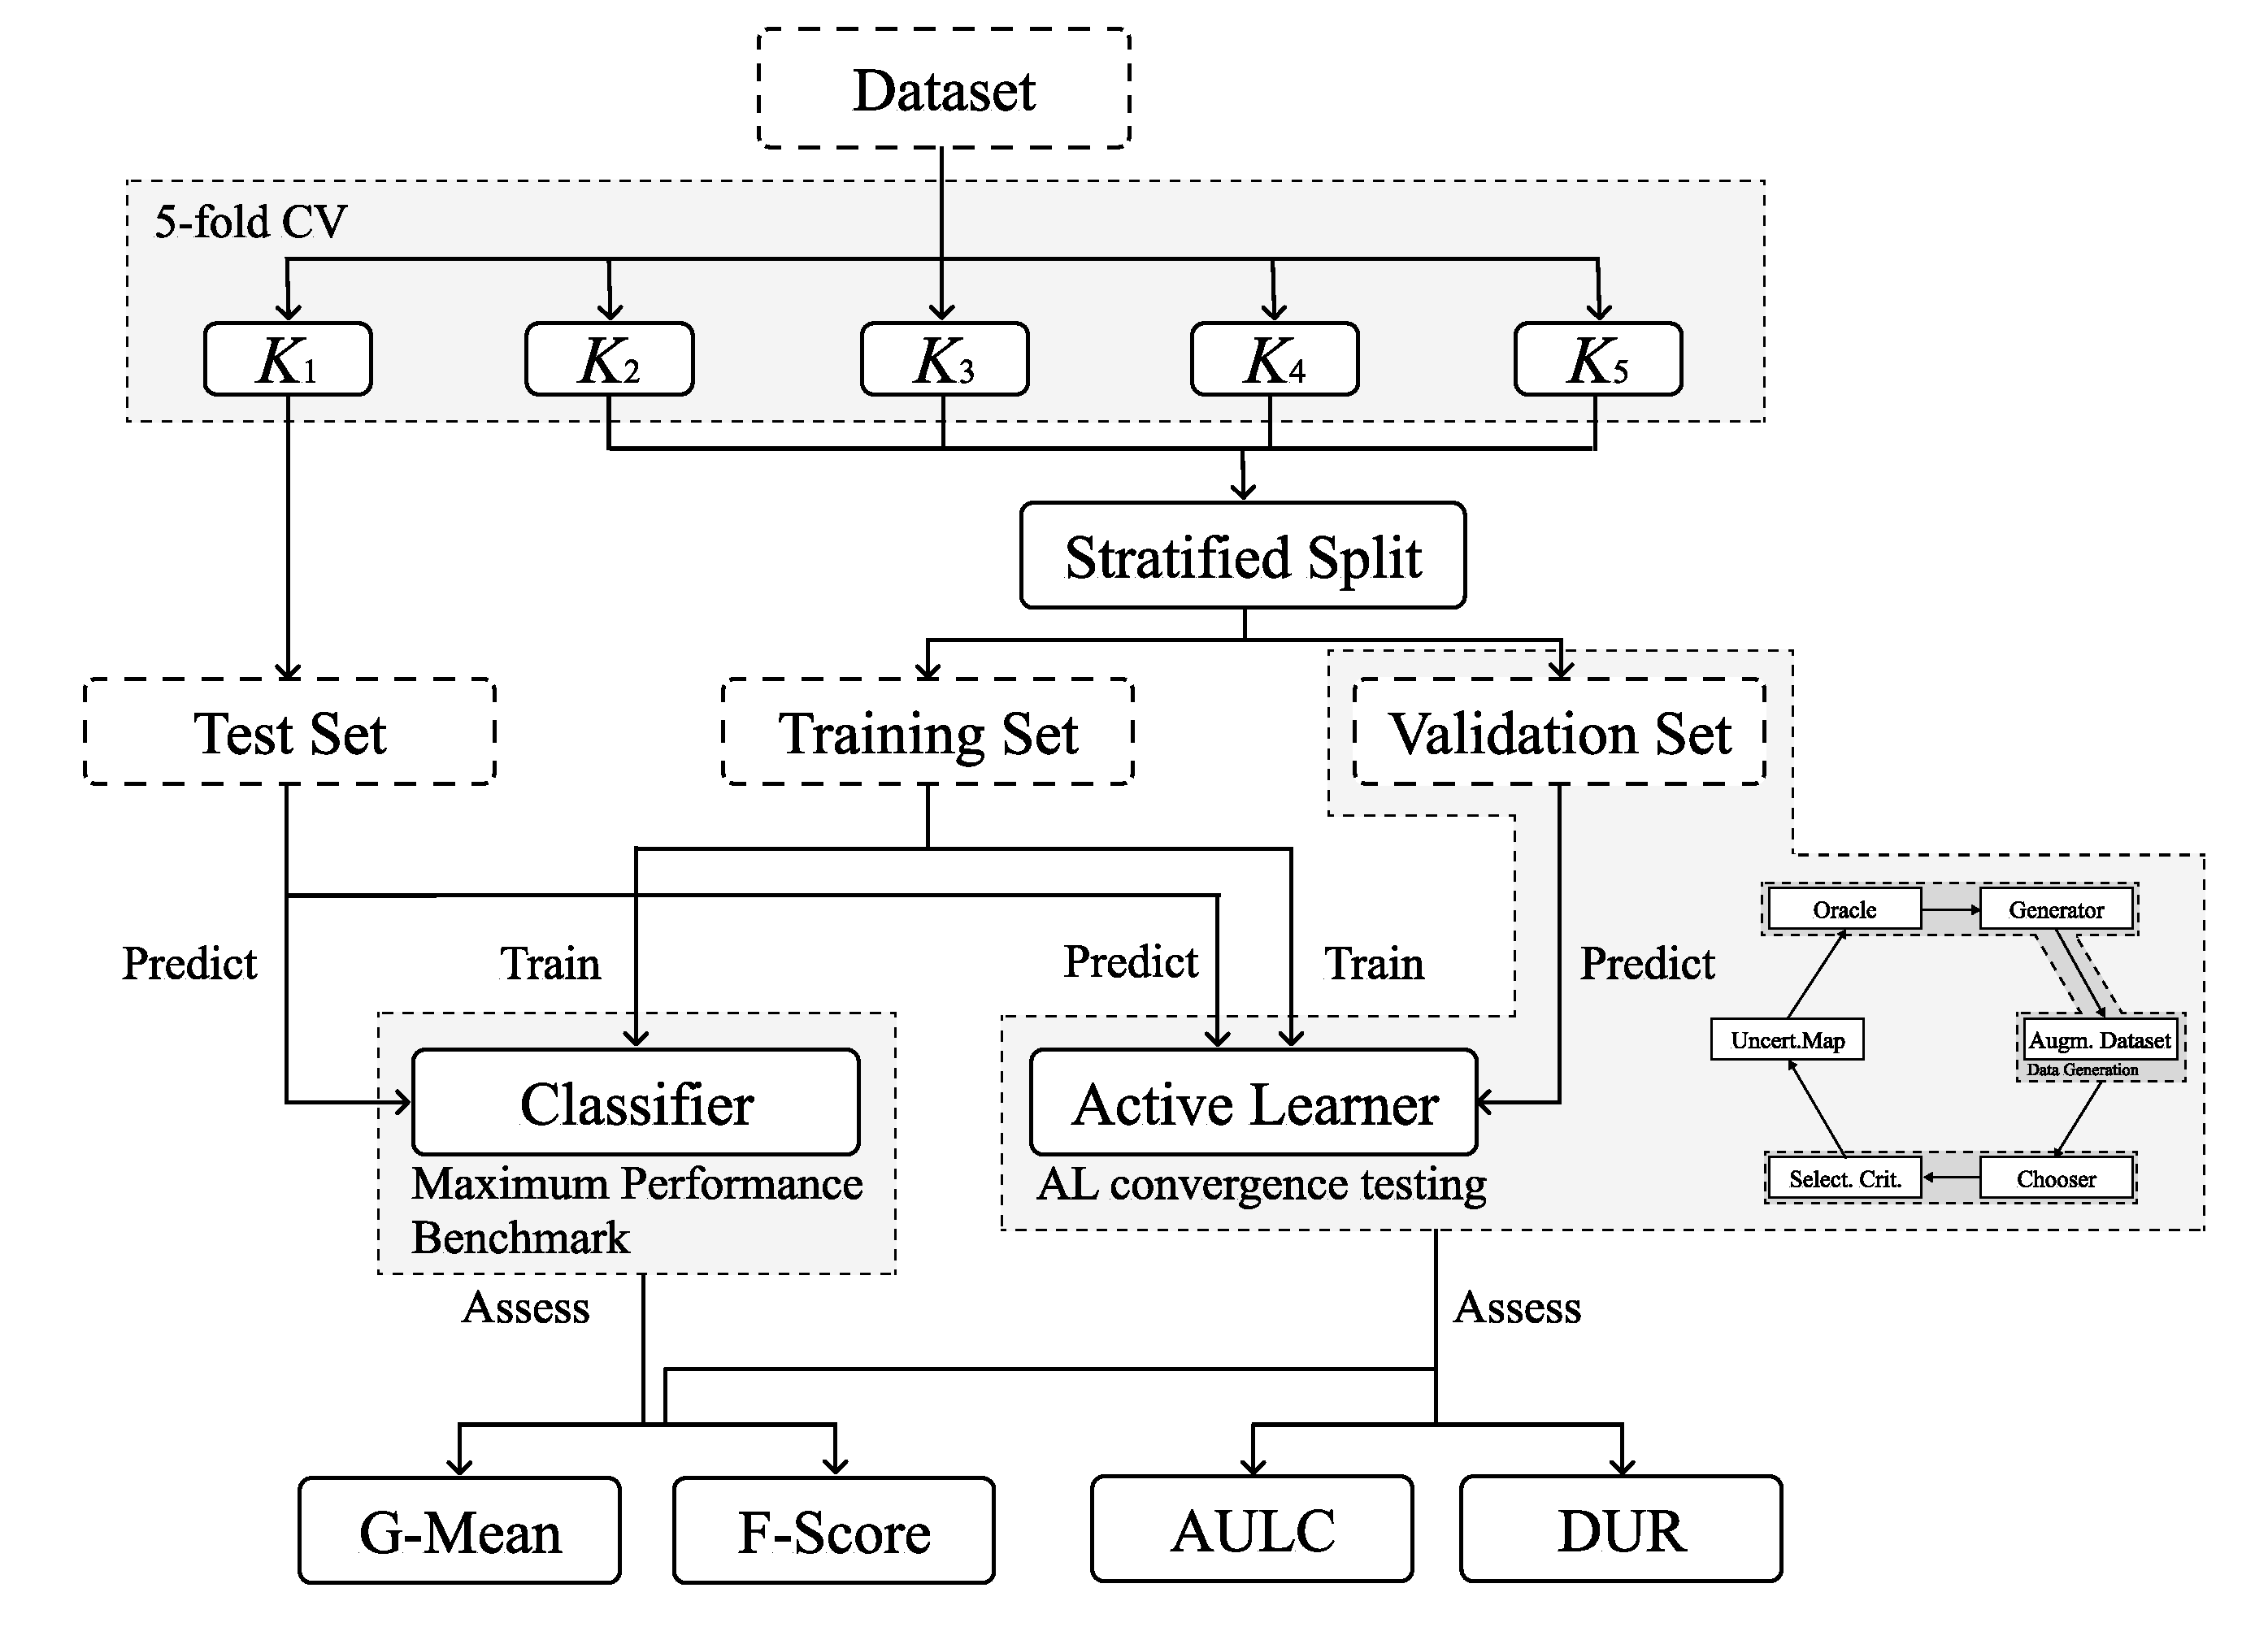
\includegraphics[width=.7\linewidth]{../analysis/experiment_pipeline}
    \caption{Experimental procedure. The performance metrics are averaged over
    the 5 folds across each of the 3 different initializations of this
    procedure for a given combination of generator, chooser/predictor and
    selection criterion.}~\label{fig:experiment_pipeline}
\end{figure}

To make the convergence metrics comparable across active learners, the
configurations of the different frameworks must be similar. For each dataset,
the number of observations is constant to facilitate the analysis of the same
metrics. 

In most practical AL applications it is assumed that the number of observations
in the initial training sample is too small to perform hyperparameter tuning.
Consequently, in order to ensure realistic results, our experimental procedure
does not include hyperparameter optimization. The predefined hyperparameters
are shown in Table~\ref{tab:grid}. They were set up based on general
recommendations and default settings for the classifiers and generators used.

The AL iterative process is set up with a randomly selected initial training
sample with 15 initial samples. At each iteration, an additional 15 samples are
added to the training set. This process is stopped after 49 iterations, once
50\% of the dataset is added to the augmented dataset.

\begin{table}[H]
	\centering
	\begin{tabular}{lll}
		\toprule
		Classifier & Hyperparameters      & Values             \\
		\midrule
		LR         & maximum iterations   & 10000              \\
		           & solver               & sag                \\
                   & penalty              & None               \\
		KNN        & \# neighbors         & 5                  \\
                   & weights              & uniform            \\
                   & metric               & euclidean          \\
		RF         & maximum tree depth   & None               \\
		           & \# estimators        & 100                \\
                   & criterion            & gini               \\
		\toprule
		Generator  &                      &                    \\
		\midrule
		SMOTE      & \# neighbors         & 5                  \\
		G-SMOTE    & \# neighbors         & 5                  \\
                   & deformation factor   & 0.5                \\
                   & truncation factor    & 0.5                \\
		\bottomrule
	\end{tabular}
    \caption{\label{tab:grid}Hyper-parameter definition for the classifiers and
    generators used in the experiment.}
\end{table}

\subsection{Software Implementation}

The experiment was implemented using the Python programming language, along
with the Python libraries
\href{https://scikit-learn.org/stable/}{Scikit-Learn}~\cite{Pedregosa2011},
\href{https://imbalanced-learn.org/en/stable/}{Imbalanced-Learn}~\cite{JMLR:v18:16-365},
\href{https://geometric-smote.readthedocs.io/en/latest/?badge=latest}{Geometric-SMOTE},
\href{https://cluster-over-sampling.readthedocs.io/en/latest/?badge=latest}{Cluster-Over-Sampling}
and
\href{https://research-learn.readthedocs.io/en/latest/?badge=latest}{Research-Learn}
libraries.  All functions, algorithms, experiments and results are provided in
the
\href{https://github.com/AlgoWit/publications/tree/master/remote-sensing/al-generator}{GitHub
repository of the project}.

\section{Results}~\label{sec:results}

The evaluation of the different AL frameworks in a multiple dataset context
should not rely uniquely on the mean of the performance metrics across
datasets.~\cite{demvsar2006} recommends the usage of mean ranking scores,
since the performance levels of the different frameworks varies according to
the data it is being used on. Consequently, evaluating these performance
metrics solely based on their mean values might lead to inaccurate analyses.
Accordingly, the results of this experiment is analysed using both the mean
ranking and absolute scores for each model.  The rank values are assigned
based on the mean scores resulting from three different initializations of
5-fold cross validation for each classifier and active learner.

Table~\ref{tab:aulc_ranks} shows the average rankings and standard deviations
across datasets of the AULC scores for each active learner. These results show
that the convergence efficiency of the proposed method (i.e., using generators
G-SMOTE and SMOTE) is consistently higher than the traditional AL framework
(NONE). With the exception of two scenarios, the proposed framework using
G-SMOTE was able to outperform the remaining methods. The only scenario where
the baseline active learner was able to outperform the remaining methods was
using the LR classifier and OA as the optimization goal. 

\pgfplotstabletypeset[
	begin table=\begin{longtable},
	end table=\end{longtable}, col sep=comma, header=true, string type, 
    every head row/.style={before row=\toprule, after row=\midrule\endhead},
	every last row/.style={after row=\bottomrule \caption{\label{tab:aulc_ranks}
	Mean rankings of the AULC metric over the different datasets used in the
    experiment.}}
]{../analysis/mean_std_aulc_ranks.csv}

The mean absolute scores are provided in Table~\ref{tab:aulc_scores}. In some
situations, there is a significant performance superiority across active
learners. The high AULC values are owed to the naturally high classification
performance of baseline methods, which makes the performance variability among
frameworks particularly meaningful. 

\pgfplotstabletypeset[
	begin table=\begin{longtable},
	end table=\end{longtable},  col sep=comma, header=true, string type, 
    every head row/.style={before row=\toprule, after row=\midrule\endhead},
	every last row/.style={
        after row=\bottomrule \caption{\label{tab:aulc_scores}
	Average AULC of each AL configuration tested.}}
]{../analysis/mean_std_aulc_scores.csv}

The mean deficiency scores of the proposed framework is shown in
Table~\ref{tab:deficiency_scores}. This metric is calculated using the proposed
framework using G-SMOTE and SMOTE as algorithms $A$ and the baseline active
learner as algorithm $B$. The proposed method shows consistent a improvement
over the baseline method, except in three situations, where the difference
among active learners is marginal.

\pgfplotstabletypeset[
	begin table=\begin{longtable},
		end table=\end{longtable},  col sep=comma, header=true,
	string type, every head row/.style={before row=\toprule, after row=\midrule\endhead},
	every last row/.style={after row=\bottomrule \caption{\label{tab:deficiency_scores}
    Mean deficiency scores. The scores were calculated by estimating the
    deficiency of the proposed framework with respect to the original AL
    framework.}}
]{../analysis/mean_std_deficiency.csv}

The average DURs are shown in Figure~\ref{fig:dur}. They were calculated for
various threshold levels, varying at a step of 5\% between 60\% and 95\%. The
DURs shown in the figure use the typical AL framework as the baseline strategy.
The results show a generalized decrease of data required to reach the
performance thresholds in the various scenarios. For higher performance
thresholds, the gap between the proposed and baseline methods tend to be
reduced, since the amount of data required is larger and the benefits of data
generation is less apparent.

\begin{figure}[H]
	\centering
	\includegraphics[width=1\linewidth]{../analysis/data_utilization_rate}
    \caption{Mean data utilization rates. The y-axis shows the average amount
    of data necessary to reach the different performance thresholds (as a
    percentage of the baseline AL framework).}~\label{fig:dur}
\end{figure}

The mean optimal classification scores is shown in
Table~\ref{tab:optimal_mean_std_scores}. The maximum performance (MP)
classification scores are shown as a benchmark and represent the performance
of the corresponding classifier using the entire training set. One of the
goals of this study is ensuring that the classification performance of the
predictors resulting from the proposed framework are not worse than the
predictors produced using the typical AL framework. Using a generator in AL's
iterative process was capable of outperforming the baseline framework in most
cases and the maximum performance classifier in 6 of those.

\pgfplotstabletypeset[
	begin table=\begin{longtable},
		end table=\end{longtable},  col sep=comma, header=true,
	string type, every head row/.style={before row=\toprule, after row=\midrule\endhead},
	every last row/.style={after row=\bottomrule
        \caption{\label{tab:optimal_mean_std_scores}
    Optimal classification scores. The Maximum Performance (MP) classification
    scores are calculated using classifiers trained using the entire training
    set.}}
]{../analysis/optimal_mean_std_scores.csv}

The optimal AULC results of each method are reported in
Table~\ref{tab:wide_optimal_aulc}. These results depict in higher detail the
findings drawn from this experiment.

\pgfplotstabletypeset[
	begin table=\begin{longtable},
		end table=\end{longtable},  col sep=comma, header=true,
	string type, every head row/.style={before row=\toprule, after row=\midrule\endhead},
	every last row/.style={after row=\bottomrule
        \caption{\label{tab:wide_optimal_aulc}
            Mean cross-validation scores of AL algorithms for each dataset.
            Legend: IP Indian Pines, KSC Kennedy Space Center, PC Pavia Center, PU
            Pavia University, SA Salinas A.}}
]{../analysis/wide_optimal_aulc.csv}

\section{Conclusion}~\label{sec:conclusion}

The aim of this experiment was to test the effectiveness of a new AL framework,
where a new element is introduced to improve the convergence rate of AL through
the use of artificial data generation. The experiment was designed to test the
proposed method under particularly challenging conditions, where the maximum
performance line is naturally high in most datasets (with exception to the
Indian Pines dataset). In order to test basic setups for this new framework,
the elements that constitute the Generator component were set up in a
plug-and-play scheme, without significant tuning of the data generators (SMOTE
and G-SMOTE). The tests showed that this new framework is able to consistently
outperform the original AL framework in most scenarios, as shown in
Table~\ref{tab:wide_optimal_aulc}. These results could be further improved
through the modification and more intense tuning of the data generation
strategy. In our experiment, during each iteration, the new artificial data is
generated only to match each non-majority class frequency with the majority
class frequency, thus strictly balancing the class distribution. Generating a
larger amount of data for all classes (especially in early iterations) can
further improve these results. 

We also consider the fast convergence of AL on these datasets. The high
performance scores for the baseline AL framework made the achievement of
significant improvements over the traditional AL framework under
these conditions particularly meaningful. The advantage of the proposed AL
framework is shown in Figure~\ref{fig:dur}. In most of the presented scenarios
there is a substantial reduction of necessary data to reach each of the tested
performance metric thresholds. 

The results from this experiment show that the inclusion of a data generator in
the AL framework will yield significant improvements in the convergence of the
method. The proposed method successfully anticipated the predictor's optimal
performance, as shown in Tables~\ref{tab:aulc_ranks},~\ref{tab:aulc_scores}
and~\ref{tab:deficiency_scores}. This means the annotation cost would have been
reduced in a real application since the number of iterations and labeled
samples necessary to reach near optimal classification performance is reduced,
as shown in Figure~\ref{fig:dur}. The class imbalance bias observed in AL tasks
is reduced, as shown in Table~\ref{tab:deficiency_scores}, where data
imbalance appropriate metrics are always improved over the baseline scores.

\bibliography{references}
\bibliographystyle{apalike}

\end{document}
